\newpage
\section{Implementierung}

Wie in Abschnitt XX bereits erwähnt ist die Applikation dem Design-Pattern Model-View-Controller nachempfunden. Im Folgenden wird nun die konkrete Implementierung beschrieben und die Architektur mittels Codebeispielen konkretisiert.
\\
Der allgemeine Ablauf der Anwendung sieht lediglich einen Aufruf der HTML-Seite index.html vor. In diese wird mittels Javascript der jeweilige Inhalt (eine View) geladen und mit Daten und Funktionen (Controller) und versorgt.
\\
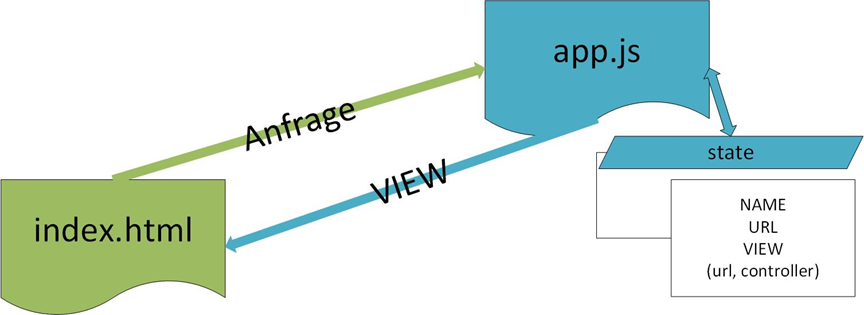
\includegraphics[width=1\textwidth]{ref/images/index.png} \\ 
App.js ist eine Javascript-Datei, die die Zuordnung der Views zu ihrem jeweiligen Controller durchführt. An dieser Stelle ist pro View ein Status (state) hinterlegt, der die folgenden Informationen definiert (Name des Status, URL (innerhalb der App), View-Bezeichnung (URL der View, Controllername)). Die Informationen über die aktuell gewählte View gibt app.js an index.html zurück, welche sie nach außen dem Nutzer darstellt.
\\
App.js wird bei jedem Start der Applikation zuerst geladen. Dabei findet auch immer eine Prüfung der aktuellen Internetverbindung statt. Internet wird für die Darstellung des Kartenmaterials benötigt. Die Konsequenz einer fehlenden Internetverbindung ist demnach ein Abbruch der Applikation.
\\
Standardmäßig wird bei korrektem Startverhalten die play-View geladen. Das ist eine ebenfalls in app.js definierte Defaulteinstellung.
\\
Alle folgenden Statusbeschreibungen trennen View, Controller und Modell schematisch voneinander, wobei der Begriff Modell durch den Cordova-spezifischen Begriff Service ersetzt wird.
\\
Die App besitzt einen getabbten Aufbau, das heißt es existiert eine Kopfzeile, die dem Nutzer vier verschiedene Tabs anbietet: Spielen, Highscores, Account und Credits. 
\\
Die in index.html angezeigten Tabs sind ein Spezialstatus, der in app.js als abstrakt gekennzeichnet ist und ständig im Hintergrund aktiv ist. Alle folgenden Tabs bauen auf diesem abstrakten Status auf.
\\
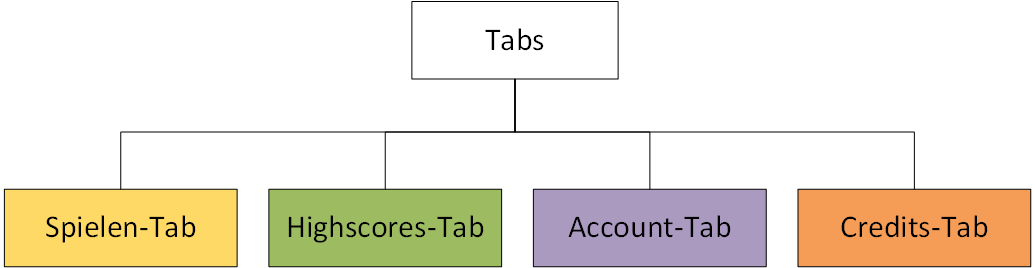
\includegraphics[width=1\textwidth]{ref/images/tabs.png} \\ 

Jeder der Tabs wird im Folgenden näher beschrieben werden.

\subsection{Spielen-Tab}
Der Spielen-Tab bietet dem Nutzer die Möglichkeit ein Spiel zu starten. Er gibt dafür einen Namen und einen Spielradius an. Unter dieser Kombination wird er später seinen Highscore dieses Spiels finden können. Die View, die dahinter steht ist die Play-View, welche prinzipiell im Spielen-Tab als Startseite der Applikation angezeigt wird. 
\subsubsection{Play-View}
%
%Beschreibung der HTML-Seite
%
Die Play-View hat ein Textfeld, dass den Spielernamen übernehmen kann und eine Selectbox, die den Radius auf zwei bis fünf Kilometern beschränkt. Bei fehlender Eingabe wird auf drei Kilometer als Defaultwert gesetzt. Außerdem bietet die View einen Button, der das Spiel startet. 
%
%Ablaufplan
%
\\ 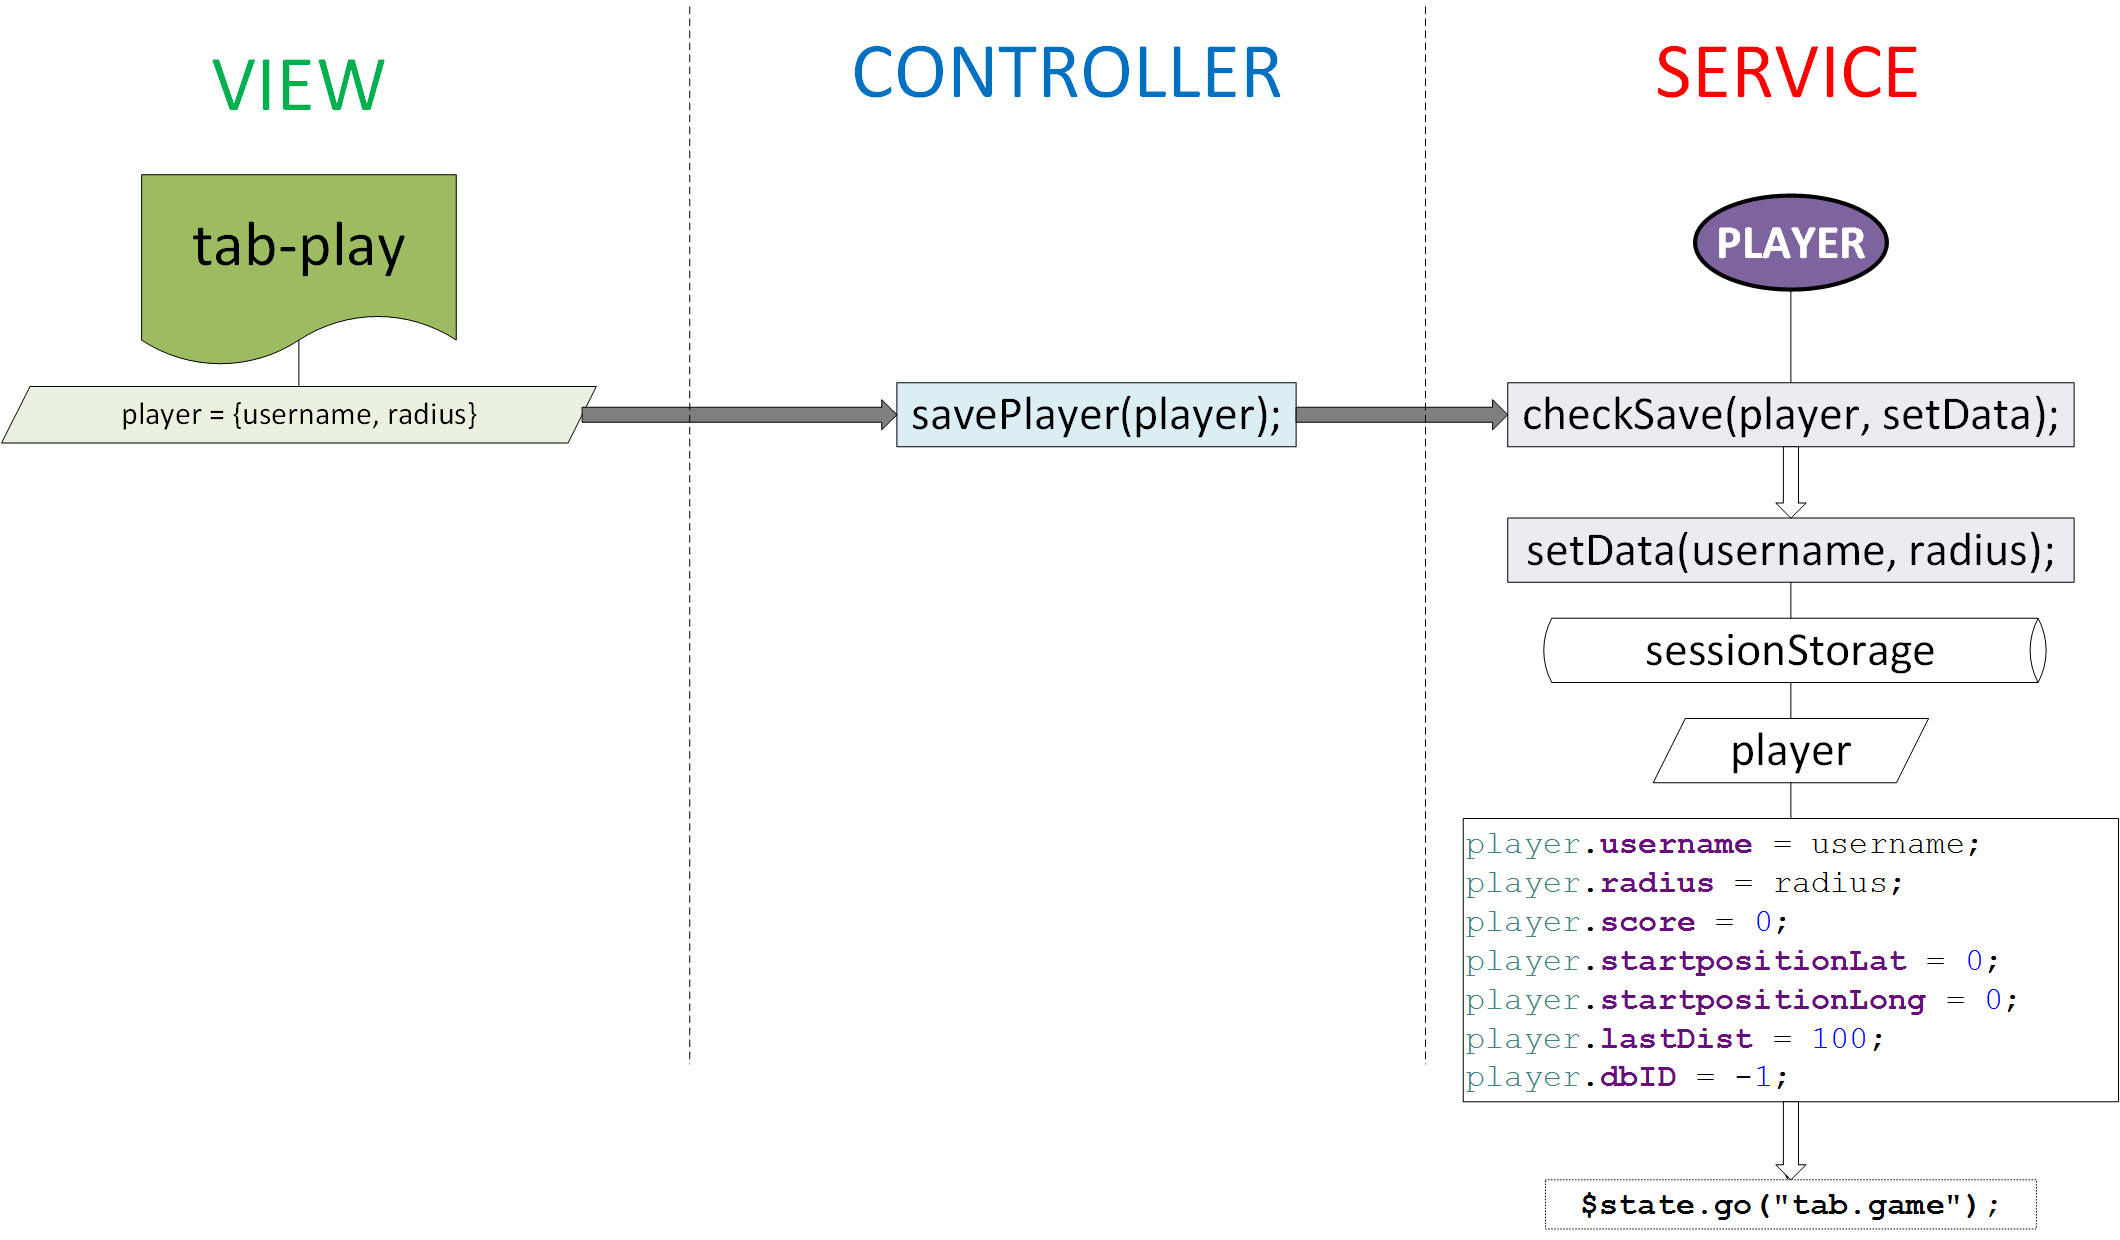
\includegraphics[width=1\textwidth]{ref/images/02-play-tab.png} \\
%
% Beschreibung des Controllers und der Services
%
Der Play-View wurde über app.js der Controller 'PlayCtrl' zugewiesen, der wiederum Zugang zum Service 'Player' besitzt. Der 'Player'-Service kapselt alle Funktionen, die mit den Nutzerdaten im Zusammenhang stehen.
\\
% Verwendungszweck
\\
Schon während der Eingabe der benötigten Informationen (Name und Radius) wird ein JS-Objekt 'player' generiert, das diese Daten enthält. Mit Druck auf den Button 'Los gehts' an die Funktion 'savePlayer' des Controllers übergeben wird. 
\\
Der Controller leitet bei Aufruf dieser Funktion die Objektdaten Name und Radius an den dazugehörigen Service 'Player', der zuerst auf gültige Befüllung des Spielernamen prüft und bei Befüllung diesen speichert. Der genutzte Speicher ist der sessionStorage des Geräts, der für die Dauer der Session die Daten des Spielers als Objekt mit den folgenden Eigenschaften speichert: 
\begin{enumerate}
\item Spielername und Radius: beides über Nutzer eingegeben und über Controller an Service zur Speicherung übergeben
\item Score: Punktestand des Spielers
\item StartpositionLat: Breitengrad der Startposition
\item startpositionLong: Längengrad der Startposition
\item lastDist: letzte Distanz zum Ziel für Verlaufsvergleich
\item dbID: ID des Spielers im Spielerarray des Sessionstorage
\item lastUpdate: Zeitpunkt der letzten Änderung
\end{enumerate}
Die noch nicht existierenden Werte werden mit Defaultwerten gefüllt.
\\
Wenn der Spielername nicht angegeben wurde erhält der Nutzer eine Aufforderung und das Spielerobjekt wird nicht weitergeleitet/gespeichert. Bei erfolgreichem Speichern hingegen erfolgt über den Service eine Weiterleitung in den Status 'tab-game'.

\subsubsection{Game-Tab}
%
%Beschreibung der HTML-Seite
%
Die Game-View liegt ebenfalls im Tab 'Spielen' und ist für die aktuelle Standortbestimmung - also die Bestimmung des Startpunkts des Nutzers zuständig.
\\
Sie besitzt anfänglich lediglich einen Button, der die Positionsbestimmung anstößt. Bei fehlerfreier Ermittlung wird dem Nutzer eine Open Street Map mit seiner Position und dem eingezeichneten Radius angezeigt, sodass er einen Überblick über sein 'Spielfeld' bekommt. Außerdem wird ein weiterleitender Button eingeblendet, über den der Spieler die Spielmöglichkeiten in seinem berechneten Umfeld angeboten erhält.
Bei Fehlern bei der Positionsbestimmung erhält der Nutzer anstelle der Karte und des Button schriftliche Rückmeldung über die Art seines Fehlers.
%
%Ablaufplan
%
\\ 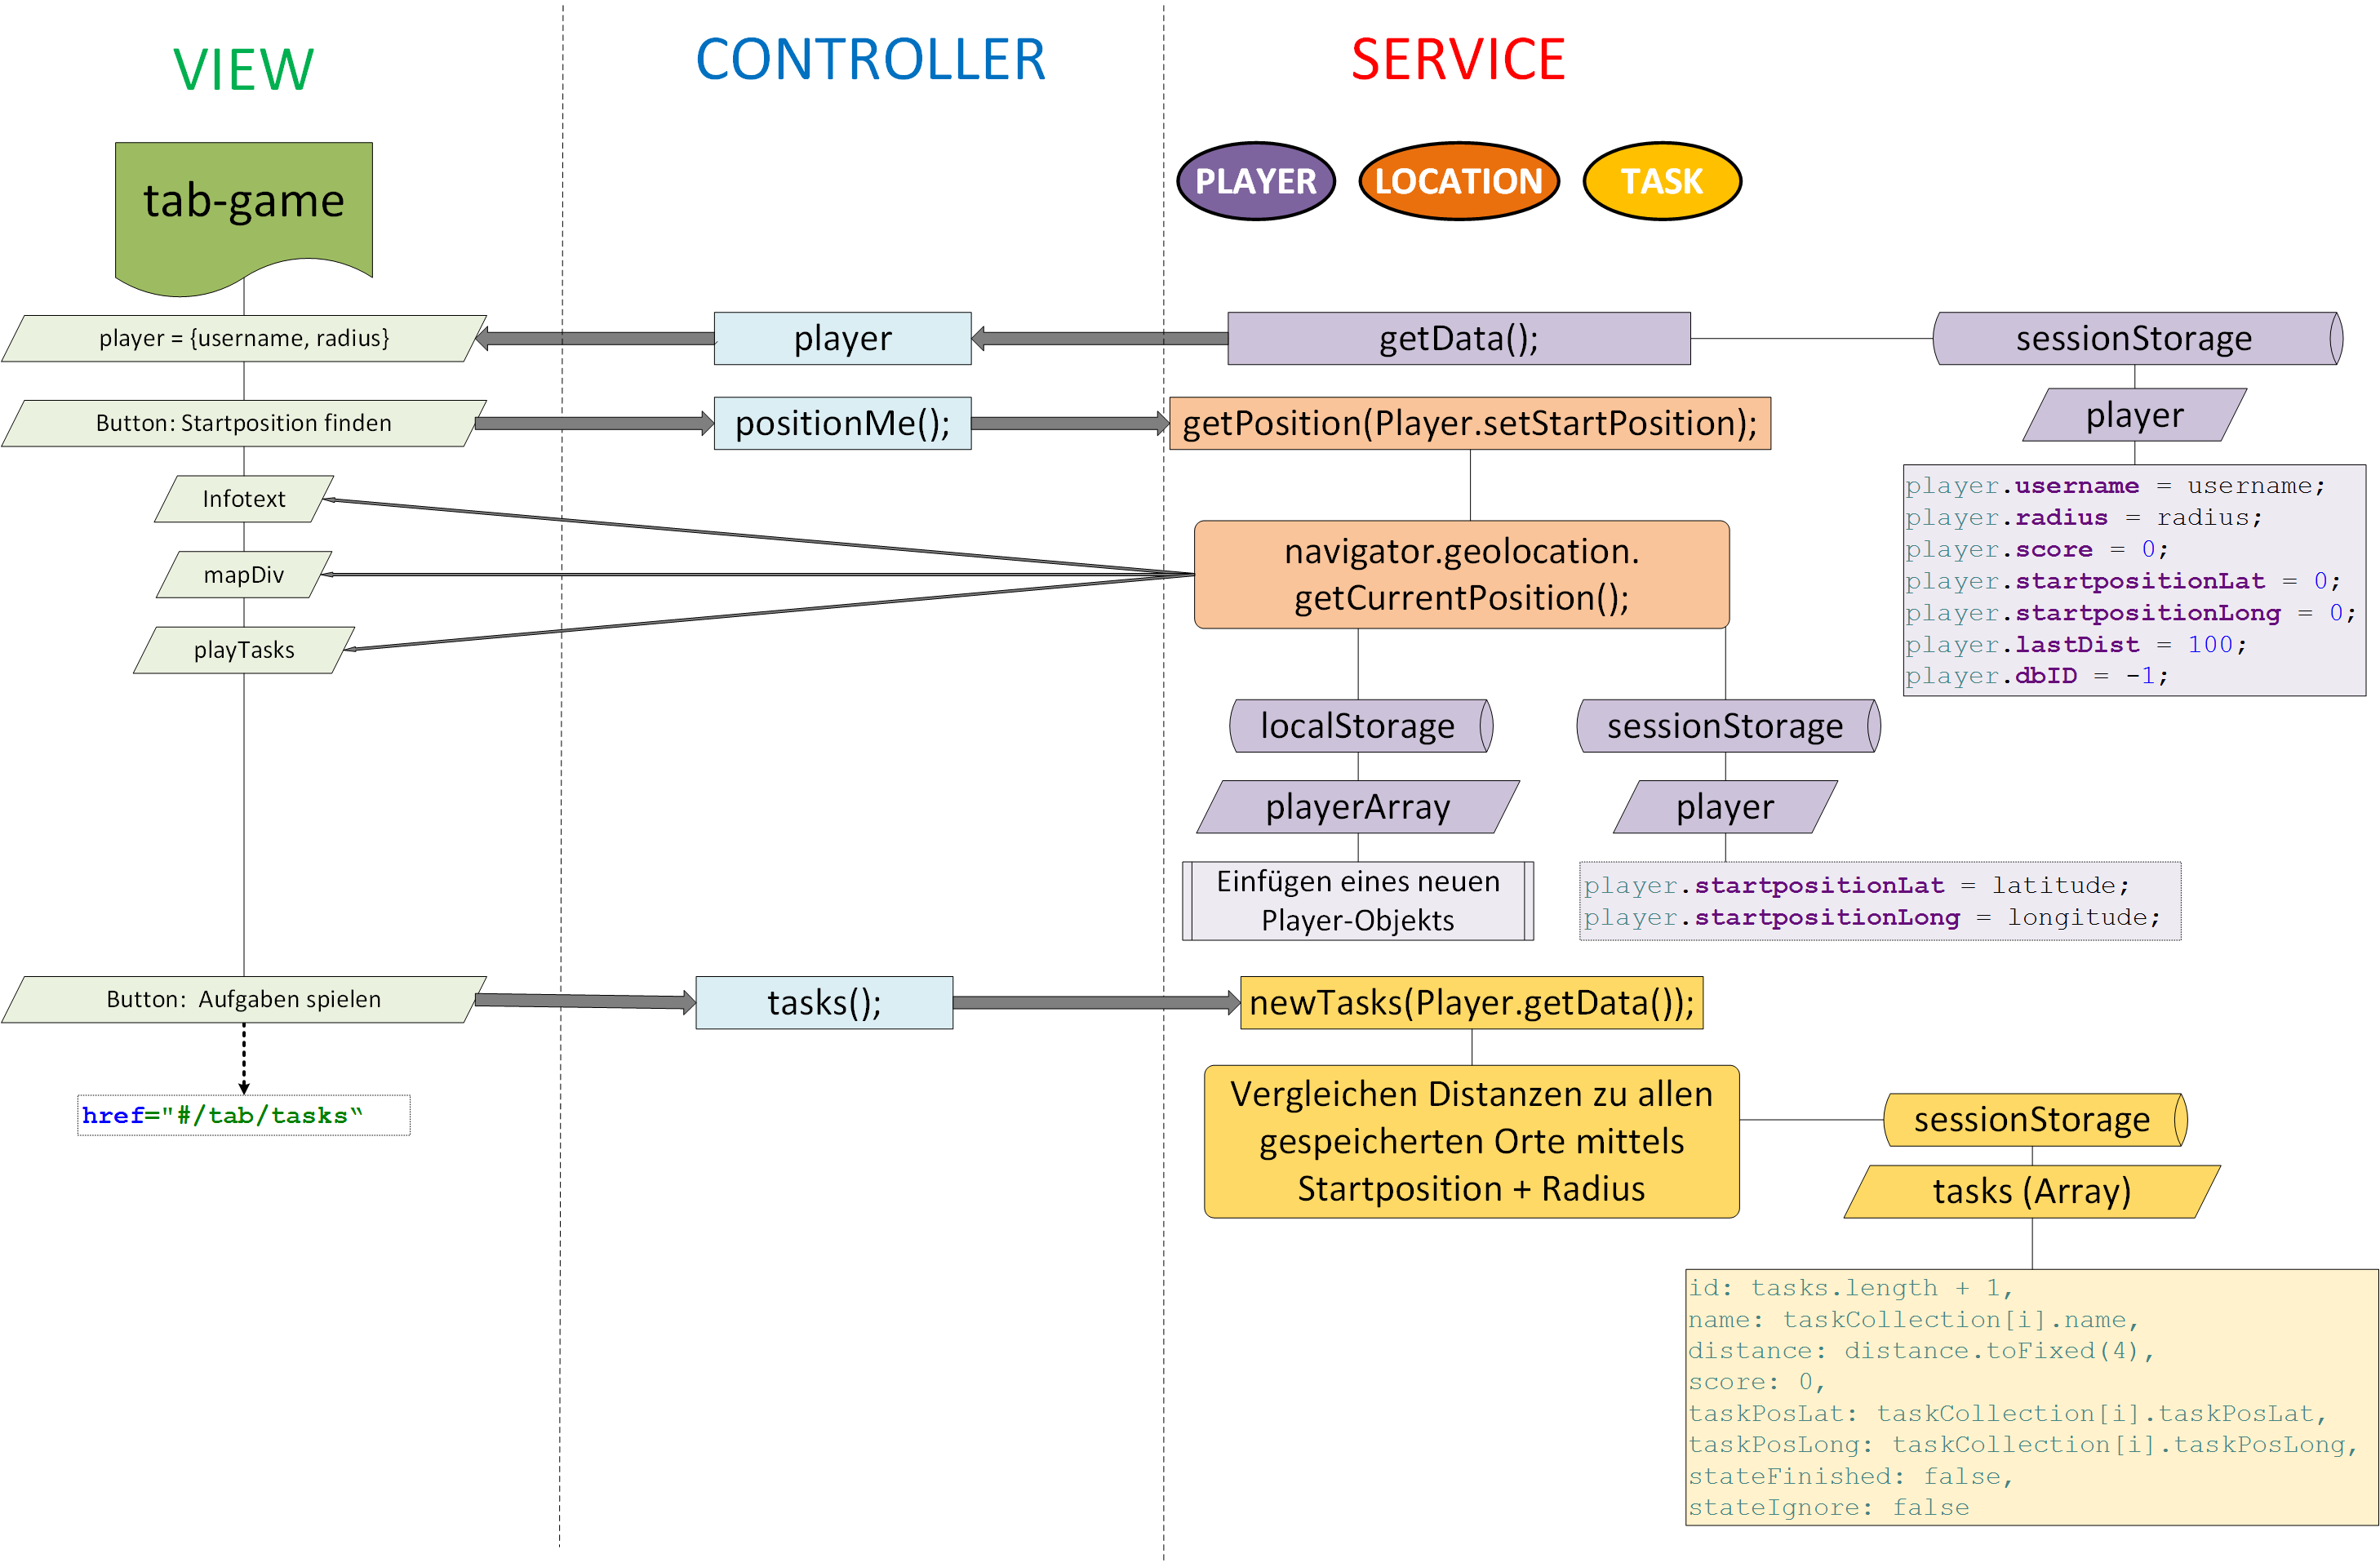
\includegraphics[width=1\textwidth]{ref/images/03-game-tab.png} \\
%
% Beschreibung des Controllers und der Services
%
Die Game-View ist an den Controller 'GameCtrl' gebunden, welcher auf drei verschiedene Services zugreifen kann: Player, Location und Task.
\\
Der Player Service kümmert sich, wie erwähnt um die Nutzerdaten. Der Location Service wurde entwickelt, um die Positionsbestimmung und die Behandlung der Koodinatendaten zu kapseln. Der Task Service hingegen gewährleistet die Generierung, Verfolgung und Speicherung der Aufgaben (Tasks) der ganzen Applikation.
\\
% Verwendungszweck
\\
Die Nutzung der Applikation sieht eine Bestimmung der Startposition eines Spielers vor Erstellung der Aufgaben vor. Der Spieler erhält auf der Game-View eine kurze Übersicht seiner bisher gemachten Angaben (Spielername und Radius). Dieser werden vom Controller vor dem endgültigen Laden der View beim Service Player angefragt (getData()). Der Player-Service muss dafür auf den sessionStorage des Geräts zugreifen und das 'player'-Objekt auslesen.
\\
\\
Nach dem Laden der View kann der Nutzer dann über den Button 'Startposition finden' seine aktuelle Position bestimmen lassen. Mit Klick auf den Button wird über den Controller, bzw. über seine Funktion 'positionMe', die Funktion des Location Service aufgerufen werden ('getPosition'). Diese Funktion ist nicht nur für die eigenliche Bestimmung der Koordinaten, sondern auch für die Speicherung jener Daten verantwortlich.
\\
Dafür werden ihr die Spielerdaten über das Objekt 'player' übergeben und die Funktion zur Speicherung der Daten als Javascript-Callback Funktion im Falle einer korrekten Ermittlung.
\\
Der Befehl 'navigator.geolocation.getCurrentPosition()' ist der Weg, um auf die Geolokationsfunktionen von Cordova, bzw. des Geräts zuzugreifen. Nach diesem Aufruf werden die Felder der Game-View (Infotext, mapDiv und playTasks) entsprechend gefüllt und bei erfolgreicher Durchführung die Startpositionsdaten des Spielers (vgl. Callbackfunktion) im sessionStorage aktualisiert und der Spieler in das Spielerarray des Localstorage integriert. Der Localstorage des Geräts enthält im Vergleich zum Sessionstorage zu jeder Zeit seine Daten und wird nicht automatisch gelöscht. Das Array enthält also alle Spieler, die dann später auch im Highscore aufgelistet werden können.
\\
Bei erfolgreicher Positionierung werden die Koordinaten über das mapDiv, einem Bereich der Game-View, in einer Open Street Map dargestellt (vgl. Kapitel XXX). Außerdem wird in diesem Fall der Button 'Aufgaben spielen' eingeblendet.
\\
\\
Wird dieser Button 'Aufgaben spielen' daraufhin gedrückt, startet der Controller die Erstellung der Aufgaben für den Spieler.
\\
In dieser prototypischen Implementierung ist nur eine fixe Anzahl von Aufgaben implementiert, die von den Entwicklern frei bestimmt wurden und in einem Array gespeichert sind.
\\
Jede Aufgabe in dieser Sammlung hat folgende Informationen:
\begin{enumerate}
\item id: Identifikationsnummer der Aufgabe
\item Name: schriftliche Bezeichnung der Aufgabe
\item taskPosLat: Aufgaben-Längengrad
\item taskPosLong: Aufgaben-Breitengrad
\end{enumerate}

Folgende beispielhaften Aufgaben sind im Prototypen implementiert.
\begin{lstlisting}
        var taskCollection = [
            {
                id: 0,
                name: "Mannheim Hbf",
                taskPosLat: 49.479904895467314,
                taskPosLong: 8.470357013095054
            },
            {
                id: 1,
                name: "Mannheim Universitaet",
                taskPosLat: 49.48373966279436,
                taskPosLong: 8.46222996711731
            },
            {
                id: 2,
                name: "Mannheim Wasserturm",
                taskPosLat: 49.48336089947494,
                taskPosLong: 8.477369150878872
            },
            {
                id: 3,
                name: "Mannheim Neckar",
                taskPosLat: 49.490776620594524,
                taskPosLong: 8.482561907531704
            },
            {
                id: 4,
                name: "Mannheim Rhein",
                taskPosLat: 49.494403359335486,
                taskPosLong: 8.456469378234829
            },{
            ...
            }]
\end{lstlisting}

\subsubsection{Umsetzung iBeacons}
Ziel der Umsetzung in dieser Arbeit ist, dass die definierten Zielpunkte der App mit jeweils einem iBeacon ausgestattet werden.Damit diese die Genauigkeit der Entfernung verbessern.
Hierfür muss die App Signale des iBeacons empfangen. Deshalb läuft während der gesamten Ortungsphase im Hintergrund ein iBeacon Scanner. Sobald dieser Scanner den gewünschten iBeacon entdeckt hat wird die Distanz zum Ziel durch den iBeacon bestimmt und nicht per GPS, dadurch wird eine höhere Genauigkeit im Zielgebiet erreicht.

Um dies zu implementieren, muss das Zielpunkt Objekt angepasst werden. Standortobjekte benötigen neben Namen und Positionen noch eine iBeacon ID sowie Major und Minor Werte.

Mit den neuen Werten sind alle Vorraussetzungen geschaffen um einen iBeacon Scanner zu implementieren. Hierfür wird das Plug-In "Cordova / Phonegap iBeacon plugin" von Peter Metz verwendet. Es ist open Source und kann von Git Hub heruntergeladen werden.

Das Plug-In enthält Schnittstellen und Funktionen zum finden von iBeacons. Hierbei werden zwei unterschiedliche Funktionalitäten geboten.


1. Monitoring von iBeacons
Beim Monitoring wird ständig überprüft ob das Smartphone welches das Plug-In nutzt in einen Bereich eintritt, indem ein iBeacon Signale sendet. Ebenfalls wird überprüft ob das Smartphone den Bereich verlässt. Diese Funktion wird in dieser Arbeit genutzt um dem User anzuzeigen, dass bei Eintritt in eine iBeacon Zone nicht mehr GPS genutzt wird, sondern die Abstandsbestimmung mit Hilfe des iBeacons erfolgt.

2. Ranging von iBeacons
Während Monitoring nur den Aus- bzw. Einritt in eine Zone überprüft, ermittelt das iBeacon Ranging alle in der nähe befindlichen iBeacons und gibt eine ungefähre Distanz zu diesen an. Diese Funktionalität wird genutzt um die Distanz zum Zielort in der App darzustellen.\cite{MonitorRange}


Im folgenden wird die Umsetzung anhand von Quellcode Beispielen erläutert:

Installation
Damit das Plug-In genutzt werden kann, muss es erst über die Console des Betreibssystem installiert werden.

Hierfür navigiert man in der Console zum Hauptordner der App. Dort führt man den Befehl:

\begin{lstlisting}
cordova plugin add https://github.com/petermetz/cordova-plugin-ibeacon.git
\end{lstlisting} 


aus. Draufhin erfolgt die Automatische Installation im Ordner "plugin" der App und es kann auf die Schnittstellen zugegriffen werden.

Der allgemeine Ablauf besteht aus mehreren Schritten:
\begin{enumerate}
\item Schritt Anlegen eines Arrays mit iBeacon Informationen
\item Schritt Hauptfunktion mit for-Schleife aufrufen
\item Schritt Warten auf einen iBeacon in Reichweite
\item Schritt Gefundenes iBeacon-Objekt in Variable schreiben
\item Schritt Daten aus Objekt auslesen und anzeigen
\end{enumerate}



\underline{TODO: An dieser Stelle wird mit Code-Listings die Umsetzung dieser Schritte }\\
\underline{detailliert erläutert werden.}
